\documentclass[12pt, a4paper, times, capchap, capsec,
floatnumber=continuous, header=yes]{abnt}
\usepackage[utf8]{inputenc} % acentos em portugues
\usepackage{graphicx} % importar imagens
\usepackage{sty/abnt-UFSC}
\usepackage{longtable,color}
\usepackage{amsmath}
\newcommand{\norm}[1]{\left\lVert#1\right\rVert}
\usepackage{amstext}
\usepackage{amsfonts}
\usepackage{amssymb}
\usepackage{array}
\usepackage{hyphenat}
\usepackage{url}
\usepackage{caption}
\usepackage{float}
\usepackage{listings}
\usepackage{textcomp}

\lstset{language=Python,
numbers=left,
stepnumber=1,
firstnumber=1,
numberstyle=\tiny,
extendedchars=true,
breaklines=true,
frame=tb,
basicstyle=\footnotesize,
stringstyle=\ttfamily,
showstringspaces=false
}
\renewcommand{\lstlistingname}{C\'{o}digo Fonte}
\renewcommand{\lstlistlistingname}{Lista de C\'{o}digos Fonte}

\def\Versao$#1 #2${#2}
\def\Data$#1 #2 #3${#2}

\autor{Vitor Arins Pinto}
\titulo{Redes Neurais Convolucionais de Profundidade para
  Reconhecimento de Textos em Imagens de CAPTCHA.}
\orientador[]{Orientadora: Luciana de Oliveira Rech }
\comentario{Trabalho de Conclusão de Curso submetido ao Programa de
  graduação da Universidade Federal de Santa Catarina para a obtenção
  do Grau de Bacharel em Sistemas de Informação.}
\instituicao{Universidade Federal de Santa Catarina \par
    Centro Tecnológico \par
    Departamento de Informática e Estatística}
\local{Florian\'{o}polis}
\data{\today}


\begin{document}

\capa
\folhaderosto

% Folha de aprovação
\begin{folhadeaprovacao}
  \begin{center}
    \large
    Vitor Arins Pinto\\[2cm]
    \espaco{simples}
    REDES NEURAIS CONVOLUCIONAIS DE PROFUNDIDADE PARA RECONHECIMENTO
    DE TEXTOS EM IMAGENS DE CAPTCHA.\\[2cm]
    \begin{espacosimples}
      Este Trabalho de Conclusão de Curso foi julgado aprovado para a
      obtenção do Título de “Bacharel em Sistemas de Informação”, e
      aprovado em sua forma final pelo Curso de Bacharelado em Sistemas de
      Informação.
    \end{espacosimples}
    \assinatura{Prof. Renato Cislaghi, Dr.\\Coordenador}
  \end{center}
  {\bf Banca Examinadora:}
  \begin{flushright} 
    \assinatura*{Prof.ª Luciana de Oliveira Rech, Dr.ª\\Orientadora}
    \assinatura*{Prof. Mário Antônio Ribeiro Dantas, Dr.}
    \assinatura*{Prof.ª Jerusa Marchi, Dr.ª}
  \end{flushright}
  \begin{center}
    \vfill
    \espaco{simples}
    Florianópolis\\
    2016
  \end{center}
  \clearpage
\end{folhadeaprovacao}

\chapter*{Agradecimentos}

Primeiramente gostaria de agradecer à minha amada namorada e melhor
amiga Letícia, que além de me mostrar o real significado do amor e
me apresentar a felicidade de uma maneira que eu não conhecia,
cooperou no desenvolvimento do trabalho desde o seu início, suportando
amorosamente a minha ausência, se sobrecarregando com trabalho
(inclusive o de revisar esse texto) permitindo que eu me dedicasse
integralmente ao desenvolvimento do mesmo.

Aos meus pais agradeço por todo o esforço e sacrifício que fizeram
para que eu pudesse chegar aqui, sem eles eu certamente não teria
oportunidade de realizar este trabalho nem de viver todas as
experiências maravilhosas que tive até hoje.

Ao meu irmão Marcel por tudo que me ensinou e todos os conselhos que
me deu até hoje.

Agradeço à Marilene Bittencourt que sempre me incentivou a ser melhor
e há muito tempo dá ensinamentos que me levam para um caminho de
sucesso.

Ao meu mentor Eduardo Bellani por me guiar nos primeiros momentos
profissionais de minha carreira e também por abrir meus olhos diante
de claras observações dessa imensidão que chamamos de vida.

Agradeço a Neoway e todos os seus funcionários pelas oportunidades que
me foram dadas e por fornecer dados indispensáveis no desenvolvimento
deste trabalho.

Por fim agradeço a todos os professores da UFSC que tive contato, em
especial a minha orientadora Prof.ª Luciana de Oliveira Rech, Dr.ª e aos
membros da banca Prof. Mário Antônio Ribeiro Dantas, Dr. e Prof.ª 
Jerusa Marchi, Dr.ª.
\begin{resumo}
        
Atualmente, muitas aplicações na Internet seguem a política de manter
alguns dados acessíveis ao público. Para isso é necessário desenvolver
um portal que seja robusto o suficiente para garantir que todas as
pessoas possam acessá-lo. Porém, as requisições feitas para recuperar
dados públicos nem sempre vêm de um ser humano. Empresas
especializadas em Big data possuem um grande interesse em fontes de
dados públicos para poder fazer análises e previsões a partir de dados
atuais. Com esse interesse, \textit{Web Crawlers} são
implementados. Eles são responsáveis por consultar fontes de dados
milhares de vezes ao dia, fazendo diversas requisições a um
\textit{website}. Tal \textit{website} pode não estar preparado para
um volume de consultas tão grande em um período tão curto de
tempo. Com o intuito de impedir que sejam feitas consultas por
programas de computador, as instituições que mantêm dados públicos
investem em ferramentas chamadas CAPTCHA (teste de Turing público
completamente automatizado, para diferenciação entre computadores e
humanos). Essas ferramentas geralmente se tratam de imagens contendo
um texto qualquer e o usuário deve digitar o que vê na imagem. O
objetivo do trabalho proposto é realizar o reconhecimento de texto em
imagens de CAPTCHA através da aplicação de redes neurais
convolucionais.

\end{resumo}

\begin{abstract}

Currently many applications on the Internet follow the policy of keeping
some data accessible to the public. In order to do this, it's
necessary to develop a portal that is robust enough to ensure that all
people can access this data. But the requests made to recover
public data may not always come from a human. Companies
specializing in Big data have a great interest in data from public
sources in order to make analysis and forecasts from current 
data. With this interest, Web Crawlers are implemented. They are
responsible for querying data sources thousands of times a day,
making several requests to a website. This website may not be
prepared for such a great volume of inquiries in a short period of
time. In order to prevent queries to be made by
computer programs, institutions that keep public data
invest in tools called CAPTCHA (Completely Automated Public
 Turing test to tell Computers and Humans Apart). These tools usually deal
with images containing text and the user must enter what he or she
sees in the image. The objective of the proposed work is to perform the
text recognition in CAPTCHA images through the application of
convolutional neural networks.

\end{abstract}


\listoffigures
\listoftables
% Para seguir um padrão, a lista de siglas fica em um arquivo
% separado e todas a suas configurações específicas são colocados
% neste arquivo.

\chapter*{Lista de abreviaturas e siglas}

\noindent
\verb"CAPTCHA" \dotfill \textit{Completely Automated Public Turing
  test to tell Computers and Humans Apart}\\
\verb"AWS" \dotfill \textit{Amazon Web Services}\\
\verb"IA" \dotfill \textit{Inteligência Artificial}\\
\verb"DCNN" \dotfill \textit{Deep Convolutional Neural Networks}\\
\verb"ReLU" \dotfill \textit{Rectified Linear Unit}\\
\verb"GPU" \dotfill \textit{Graphical Processing Unit}\\
\verb"GPGPU" \dotfill \textit{General Purpose Graphical Processing
  Unit}\\
\verb"MNIST" \dotfill \textit{Mixed National Institute of Standards
  and Technology}\\
\verb"RAM" \dotfill \textit{Random Access Memory}\\
\verb"ASCII" \dotfill \textit{American Standard Code for Information
  Interchange}\\
\verb"RGB" \dotfill \textit{Red Green Blue}\\

\sumario

\setcounter{page}{1}

\chapter{Introdução}

Redes neurais artificiais clássicas existem desde os anos 60, como fórmulas  
matemáticas e algorítimos. Atualmente os programas de aprendizado de máquina  
contam com diferentes tipos de redes neurais. Um tipo de rede neural muito  
utilizado para processamento de imagens é a rede neural convolucional de  
profundidade. O trabalho em questão tratará da utilização e
configuração de uma rede neural convolucional de profundidade para
reconhecimento de textos em imagens específicas de CAPTCHAs.

\section{Problema}

Com o aumento constante na quantidade de informações geradas e 
computadas atualmente, percebe-se o surgimento de uma necessidade de tornar
alguns tipos de dados acessíveis a um público maior. A fim de gerar
conhecimento, muitas instituições desenvolvem portais de acesso para
consulta de dados relevantes a cada pessoa. Esses portais, em forma de
aplicações na Internet, precisam estar preparados para receber
diversas requisições e em diferentes volumes ao longo do tempo.

Devido a popularização de ferramentas e aplicações especializadas em Big
data, empresas de tecnologia demonstram interesse em recuperar grandes
volumes de dados de diferentes fontes públicas. Para a captura de tais
dados, \textit{Web crawlers} são geralmente implementados para a
realização de várias consultas em aplicações que disponibilizam dados
públicos.

Para tentar manter a integridade da aplicação, as organizações que possuem  
estas informações requisitadas investem em ferramentas chamadas CAPTCHA  
(teste de Turing público completamente automatizado para diferenciação entre  
computadores e humanos). Essas ferramentas frequentemente se tratam de  
imagens contendo um texto qualquer e o usuário precisa digitar o que vê na  
imagem. 

O trabalho de conclusão de curso proposto tem a intenção de retratar a  
ineficiência de algumas ferramentas de CAPTCHA, mostrando como redes neurais  
convolucionais podem ser aplicadas em imagens a fim de reconhecer o texto  
contido nestas imagens. 

\section{Objetivos}

\subsection{Objetivo geral}

Analisar o treinamento e aplicação de redes neurais convolucionais de
profundidade para o reconhecimento de texto em imagens de CAPTCHA.

\subsection{Objetivos específicos}

\begin{itemize}
        \item Estudar trabalhos correlatos e analisar o estado da arte;
	\item Entender como funciona cada aspecto na configuração de
          uma rede neural convolucional;
	\item Realizar o treinamento e aplicação de uma rede neural
          artificial para reconhecimento de CAPTCHAs.
\end{itemize}

\section{Escopo do trabalho}

O escopo deste trabalho inclui o estudo e análise de uma rede neural
convolucional de profundidade para reconhecimento de texto em imagens de 
um CAPTCHA específico.

Não está no escopo do trabalho:

\begin{itemize}
  \item Analisar outras formas de inteligência no reconhecimento de
    texto. 
  \item O estudo, análise ou implementação da aplicação de redes
    neurais convolucionais para outros tipos de problemas. 
  \item O estudo, análise ou implementação de softwares do tipo
    ``crawler'' ou qualquer programa automatizado para recuperar
    quaisquer informações de websites públicos.
  \item A análise e comparação de diferentes técnicas ou parâmetros
    para otimização de redes neurais.
\end{itemize}

\section{Metodologia}

Para realizar o proposto, foram feitas pesquisas em base de dados tais
como IEE Xplorer e ACM Portal. Adquirindo assim maior conhecimento
sobre o tema, estudando trabalhos relacionados. 

Com base no estudo do estado da arte, foram feitas pesquisas e
estudos para indicar caminhos possíveis para desenvolvimento da
proposta de trabalho.

\section{Estrutura do trabalho}

Para uma melhor compreensão e separação dos conteúdos, este trabalho
está organizado em 6 capítulos. Sendo este o capítulo 1 cobrindo a
introdução ao tema, citando os objetivos e explicando a proposta.

O capítulo 2 apresenta a fundamentação teórica, com as definições das
abordagens de desenvolvimento de aprendizado de máquina e redes
neurais. Também são apresentados alguns conceitos de tipos de redes
neurais.

No capítulo 3 está a proposta de experimento a ser realizado. Assim
como uma breve ideia dos resultados esperados e a forma de avaliação
dos mesmos.

O capítulo 4 contém as informações do desenvolvimento do treinamento
da rede neural para reconhecimento de imagens de CAPTCHA.

No capítulo 5 são apresentados os testes do treinamento da rede neural
para reconhecimento de imagens de CAPTCHA. Também a apresentação dos
dados obtidos através das metodologias escolhidas no capítulo 4.

Por fim, no capítulo 6 estão as conclusões obtidas através dos
resultados deste trabalho, as vulnerabilidades que podem comprometer o
acesso à dados públicos disponbilizados e as sugestões para trabalhos
futuros relacionados.
\chapter{Fundamentação Teórica}

\section{Aprendizado de máquina}

Aprendizado de máquina, ou \textit{Machine Learning}, é uma área da
computação que emergiu de estudos relacionados ao reconhecimento de
padrões e inteligência artificial. Nesta área é contemplado o estudo e
implementação de algoritmos que conseguem aprender e fazer previsões
baseadas em dados. Esses algoritmos funcionam através da construção de
um modelo preditivo que tem como entrada um conjunto de treinamento
com dados de observações quaisquer. Desse modo as previsões são feitas
orientadas aos dados e não a partir de instruções estáticas de um
programa.

\section{Redes Neurais}

Diante das ferramentas disponíveis que tratam de aprendizado de
máquina, uma delas é a rede neural artificial.

Redes neurais artificiais são conjuntos de modelos inspirados por
redes neurais biológicas, usados para aproximar funções que dependem
de um número muito grande de entradas. De acordo com Mackay\cite{Mackay},
Redes neurais geralmente são especificadas utilizando 3 coisas:

\begin{itemize}

\item {\bf Arquitetura:} Especifica quais variáveis estão envolvidas
  na rede e quais as relações topológicas. Por exemplo, as variáveis
  envolvidas em uma rede neural podem ser os pesos das conexões entre
  os neurônios.

\item {\bf Regra de atividade:} A maioria dos modelos de rede neural
  tem uma dinâmica de atividade com escala de tempo curta. São regras
  locais que definem como as \textit{atividades} de neurônios mudam em
  resposta aos outros. Geralmente a regra de atividade depende dos
  parâmetros da rede.

\item {\bf Regra de aprendizado:} Especifica o modo com que os pesos
  da rede neural muda conforme o tempo. O aprendizado normalmente toma
  uma escala de tempo maior do que a escala referente a dinâmica de
  atividade. Normalmente a regra de aprendizado dependerá das
  \textit{atividades} dos neurônios. Também pode depender dos valores
  que são objetivos definidos pelo usuário e valores iniciais dos
  pesos.

\end{itemize}

Tomando imagens como exemplo, uma rede neural para reconhecimento de
texto pode ter como entrada o conjunto de pixels da imagem. Depois de
serem atribuídos os pesos para cada item da entrada, os próximos
neurônios serão ativados mediante a função de atividade
pré-definida. Os pesos são recalculados através da regra de
aprendizado e todo processo é repetido até uma condição determinada
pelo usuário.

\section{Convoluções}

Para entender redes neurais convolucionais, é necessário primeiro
entender o que são convoluções. Segundo Olah\cite{Olah}, uma
convolução pode ser vista como um somatório das probabilidades de
resposta de duas funções algébricas. Tendo como definição padrão de
convolução a seguinte expressão:

\begin{equation}
   (f*g)(c) = \sum\limits_{a}f(a)\cdot g(c-a)
\end{equation}

Onde {\bf \emph{f}} e {\bf \emph{g}} são duas funções, {\bf \emph{c}}
é o parâmetro de entrada para a função final e {\bf \emph{a}} é um
parâmetro de entrada escolhido para uma das funções, geralmente uma
diferença temporal.

Como podemos considerar que imagens são funções bidimensionais, é
comum realizar transformações por meio de convoluções. Estas
convoluções são executadas com uma função local pequena chamada de
``kernel''.

\begin{figure}[H]
\centering
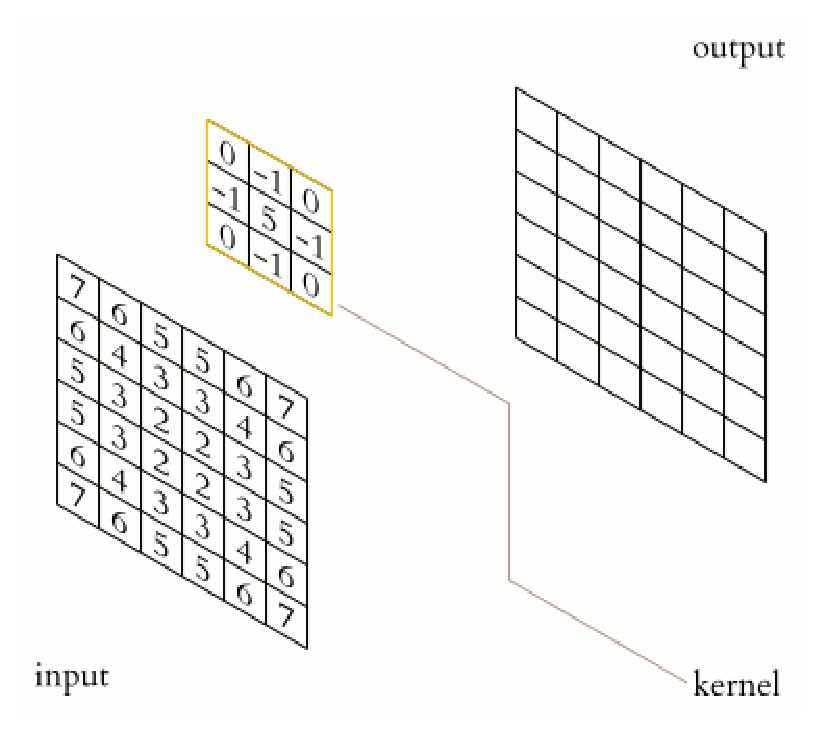
\includegraphics[scale=0.6]{imagens/fig1.eps}
\caption{Aplicação de uma função ``kernel'' sobre a função de uma
  imagem que é o ``input''.}
\label{fig:convolution_kernel}
\end{figure}

\subsection{Aplicação em redes neurais}

Redes neurais convolucionais são muito similares a redes neurais
comuns. De acordo com Karpathy\cite{Karpathy}:
\begin{quote}
  ``Arquiteturas de redes convolucionais assumem explicitamente que as
  entradas são imagens, o que nos permite cifrar algumas propriedades
  dentro da arquitetura. Essas então fazem a função de ativação mais
  eficiente de implementar e reduz drasticamente a quantidade de
  parâmetros na rede.'' (KARPATHY, 2015, tradução nossa).
\end{quote}

Portanto para o caso de reconhecimento de texto em imagens, as redes
neurais convolucionais fazem muito sentido.

\section{Aprendizado em profundidade}

O aprendizado em profundidade permite que modelos computacionais
compostos por múltiplas camadas de processamento possam aprender
representações de dados com múltiplos níveis de abstração\cite{LeCun}.

A solução de \textit{Deep learning} permite que computadores aprendam
a partir de experiencias e entendam o mundo em termos de uma
hierarquia de conceitos, com cada conceito definido em termos da sua
relação com conceitos mais simples. Juntando conhecimento de
experiência, essa abordagem evita a necessidade de ter operadores
humanos especificando formalmente todo o conhecimento que o computador
precisa. A hierarquia de conceitos permite que o computador aprenda
conceitos complexos construindo-os à partir de conceitos mais
simples. Desenhando um gráfico que mostra como esses conceitos são
construídos em cima de outros, o gráfico fica profundo, com muitas
camadas. Por esta razão, essa abordagem para IA é chamada de
Aprendizado em profundidade\cite{Goodfellow-et-al-2016-Book}.

\section{Redes neurais convolucionais de profundidade}

Ao combinar o aprendizado em profundidade com redes convolucionais,
conseguimos tratar problemas muito mais complexos de classificação em
imagens. Assim problemas mais simples, como o reconhecimento de
textos, podem ser resolvidos cada vez mais rápido e facilmente.

A grande vantagem na abordagem de redes neurais convolucionais de
profundidade (DCNN) para reconhecimento é que não é necessário um
extrator de características desenvolvido por um ser humano. Nas
soluções de \cite{Krizhevsky} e \cite{Goodfellow} é possível perceber
que foram usadas diversas camadas para o aprendizado das
características.

Em arquiteturas de profundidade, as funções de ativação dos neurônios
são unidades lineares retificadas (ReLU). Isso simplifica o uso de
\textit{backpropagation} e evita problemas de saturação, fazendo o
aprendizado ficar muito mais rápido.

\begin{figure}[H]
\centering
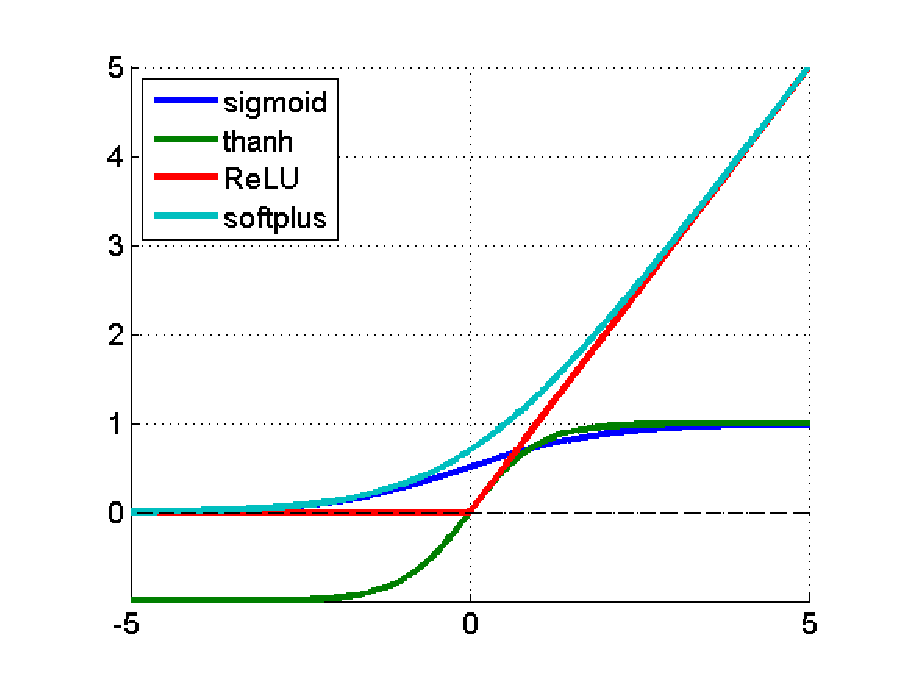
\includegraphics[scale=0.6]{imagens/activation_funcs.eps}
\caption{Comparação de funções de ativação.}
\label{fig:activation_funcs}
\end{figure}

DCNNs são a primeira abordagem verdadeiramente bem sucedida em
aprendizado em profundidade onde muitas camadas de uma hierarquia são
treinadas com sucesso de uma maneira robusta. Uma DCNN é uma escolha
de topologia ou arquitetura que se aproveita de relações espaciais
para reduzir o número de parâmetros que devem ser aprendidos, e assim
melhora o treinamento diante de uma rede com \textit{feed-forward
  backpropagation}\cite{Arel2010}.

\chapter{Proposta de experimento} \label{proposta}

Para realizar o experimento será necessário treinar um modelo de rede
neural que seja capaz, ou esteja próximo, de decifrar um CAPTCHA. Para
isso serão efetuadas três etapas básicas e comuns quando se trabalha
com redes neurais. Primeiro será coletado o maior número possível de
imagens de CAPTCHA. Em seguida será gerado um \textit{dataset} com as
características dessas imagens junto com a classe em que pertence. A
partir daí é possível realizar a configuração e treinamento da rede
neural. E por fim será calculada a acurácia, mediante imagens de
teste, do modelo que teve a melhor performance no treinamento.

\section{Coleta de imagens}

Como o escopo do trabalho não contempla a automatização da recuperação
de informações de \textit{websites} públicos, foi disponibilizado um
repositório com as imagens necessárias. Esse repositório possui
206.564 imagens e foi disponibilizado pela empresa Neoway. As imagens
se tratam de um CAPTCHA publicado pelo site do SINTEGRA de Santa
catarina
(\url{http://sistemas3.sef.sc.gov.br/sintegra/consulta_empresa_pesquisa.aspx}).

\begin{figure}[H]
\centering

\includegraphics[scale=1]{imagens/exemplo_captcha}
\caption{Um exemplo do CAPTCHA utilizado pelo sistema de consulta do
  SINTEGRA de Santa Catarina.}
\label{fig:exemplo_captcha}
\end{figure}


\subsection{Fonte pública}

Para demonstrar a ineficiência de certas imagens de CAPTCHA foi
escolhido um software Web. Este software do SINTEGRA, fornece dados
públicos de contribuintes mediante consulta via website. O SINTEGRA é
o Sistema Integrado de Informações sobre Operações Interestaduais com
Mercadorias e Serviços. Esta fonte pública possui dados fornecidos
pelos próprios contribuintes na hora do cadastro. Os comerciantes ou
profissionais autônomos fazem seu cadastro para facilitar o comércio
de produtos e prestação de serviços. O cadastro contempla inscrição da
pessoa física ou jurídica, endereço e informações complementares
referentes ao fisco estadual.

\section{Geração do Conjunto de dados}

O conjunto de dados (ou \textit{``dataset''}) que alimenta a rede neural é
gerado em tempo de execução do treinamento. Cada imagem é lida de seu
diretório em disco e carregada na memória como uma matriz de valores
de pixel. Ao final deste processo há um vetor em memória com todas
imagens existentes já pré-processadas. Isso é feito para o \textit{dataset} de
treinamento e de teste. O \textit{dataset} de treinamento terá a maioria das
imagens, que significa {\bf 180 mil} imagens para o contexto do
trabalho.

\subsection{Pré-processamento}

A fase de pré-processamento das imagens é mínima e é feita junto com a
geração do conjunto de dados.

\begin{itemize}
\item{\bf Escala de cinza}

Ao gerar um \textit{array} representativo da imagem, apenas é
considerado um valor de escala de cinza da imagem, assim padronizando
os valores de intensidade de pixels entre 0 e 1.

\item{\bf Redimensionamento}

Ao gerar o \textit{array} que representa a imagem, é feito um cálculo
para diminuir a imagem com base em uma escala. Essa escala será
configurada à partir de um valor padrão para a largura e altura das
imagens. 

\end{itemize}

\subsection{Conjunto de dados de teste}

Para o treinamento será necessário um conjunto separado para teste que
não possui nenhuma imagem presente no conjunto de treinamento.
O \textit{dataset} de testes terá uma amostra bem menor que o conjunto de
treinamento, portanto terá {\bf 8 mil} imagens.

\section{Treinamento}

Após gerado o conjunto de dados, é possível trabalhar no treinamento
do modelo da rede neural. Para isso será usado o \textit{framework}
{\bf \emph{TensorFlow}}\cite{TensorFlow} destinado à \textit{Deep
  Learning}. Também será desenvolvido um \textit{script} em
\textit{Python} que fará uso das funções disponibilizadas pela
biblioteca do \textit{TensorFlow}. Assim realizando o treinamento até
atingir um valor aceitável de acerto no conjunto de teste. O resultado
do treinamento será um arquivo binário representando o modelo que será
utilizado para avaliação posteriormente.

\subsection{Infraestrutura}

Com o intuito de acelerar o processo, foi utilizada uma
máquina com {\bf GPU} para o treinamento. A máquina foi adquirida em
uma \textit{Cloud} privada virtual da AWS\cite{GPUinstance}. A GPU
utilizada se trata de uma \textit{NVIDIA K80} com 2.496 cores e 12GB
de memória de vídeo. Como processador a máquina possui um
\textit{Intel Xeon E5-2686v4 (Broadwell)} com 4 cores, e ainda
possui 61GB de memória RAM.

\subsection{Bibliotecas utilizadas}

Todo o código foi implementado utilizando a linguagem de programação
{\bf \emph{Python}}, e as seguintes bibliotecas foram utilizadas:

\begin{itemize}

\item {\bf TensorFlow}\cite{TensorFlow}: Um \textit{framework}
  implementado em \textit{Python} destinado à \textit{Deep
    Learning}. Proporciona a criação da arquitetura e automatização do
  processo de treinamento de redes neurais com
  \textit{backpropagation}.

\item {\bf NumPy}\cite{NumPy}: Uma biblioteca em \textit{Python}
  criada para computação científica. Possui um objeto de
  \textit{array} com várias dimensões e várias funções sofisticadas
  para cálculos com algebra linear.

\item {\bf OpenCV}\cite{OpenCV}: Uma biblioteca, implementada em
  C/C++, destinada à computação visual. Utilizada para ler imagens em
  disco e realizar o pré-processamento nas mesmas.

\end{itemize}

\section{Avaliação de acurácia}

Para a avaliação, uma nova amostra de imagens será coletada do mesmo
modo que foram coletadas as imagens para treinamento. Essa amostra
terá uma quantidade maior de imagens do que o conjunto de teste.

Com essa amostra de imagens, será feita a execução do teste do modelo
contra cada uma das imagens, assim armazenando uma informação de erro
ou acerto do modelo. Ao final da execução será contabilizado o número
de acertos e comparado com o número total da amostra de imagens para
avaliação. Resultando assim em uma porcentagem que representa a
acurácia do modelo gerado.


\chapter{Desenvolvimento e Testes}

Este capítulo descreve o desenvolvimento do projeto proposto. O
projeto é composto da implementação do processador do conjunto de
dados, da implementação do script que monta e treina a rede neural e
da configuração da rede neural para otimização dos resultados. No
início foi utilizado como base um código já existente destinado ao
reconhecimento de dígitos em imagens. A partir daí foi construído o
reconhecedor textos do trabalho.

\section{Código fonte utilizado como base}

Como base da implementação deste trabalho, foi utilizado um exemplo
de código aberto disponível no repositório de códigos do
\textit{TensorFlow}\cite{mnistCode}. O código em questão seria para
reconhecer os dígitos da base dados MNIST\cite{mnist}.

O reconhecedor utilizado como base funciona apenas para dígitos
isolados em imagens separadas. Para o caso do trabalho em questões
precisaremos adaptá-lo para reconhecer conjuntos com 5 dígitos ou
letras em uma mesma imagem sem passar por um processo de segmentação
antes do treinamento.

\section{Leitura e pré-processamento do conjunto de dados}

Para a leitura das imagens e pré-processamento do conjunto de dados, foi
implementada uma classe chamada \textit{OCR\_data}. Esta classe utiliza
a memória RAM para armazenar o conjunto de dados enquanto é processado
pelo treinamento. Para Inicialização da classe, são necessários alguns
parâmetros:

\begin{itemize}

  \item Número de imagens que deve ser lido do disco.
  \item Diretório onde as imagens estão disponíveis.
  \item Número de classes que um caractere pode ter. Para o caso do
    trabalho esse número é igual a 36 pois cada caractere do CAPTCHA
    utilizado como exemplo pode ser somente uma letra minúscula sem
    acentos de ``a'' à ``z'' (26 letras) ou um número de ``0'' à ``9''
    (10 dígitos).
  \item Tamanho da fração dos dado para cada iteração com treinamento.
  \item Tamanho da palavra contida no CAPTCHA. 5 para nosso caso.
  \item Altura da imagem. Número fixo em 60 para as imagens disponíveis.
  \item Largura da imagem. Número fixo em 180 para as imagens
    disponíveis.
  \item Altura definida para redimensionamento da imagem.
  \item Largura definida para redimensionamento da imagem.
  \item A quantidade de canais de cor.

\end{itemize}

\subsection{Leitura das imagens}

As imagens são carregadas utilizando \textit{OpenCV}\cite{OpenCV} com
o método \textit{imread}. Após a leitura precisamos fixar o seu rótulo
para a utilização no treinamento. Como as imagens já estão nomeadas
com o respectivo conteúdo da sua imagem, só o que precisamos fazer é
um vetor utilizável desse texto. 

Primeiro transformamos cada caractere em um número de 0 à 35. Fazemos
isso recuperando o código ASCII de cada caractere e normalizando a
sequência. Portanto, para os dígitos (0 à 9) que possuem códigos indo
de 48 à 57, subtraímos 48. E para as letras (a à z) que possuem
códigos indo de 97 à 122, subtraímos 87 e ficamos com números de 10 à
35. 

Depois de traduzido o caractere para um número, precisamos criar o
vetor do rótulo através do nosso algoritmo de \textit{One-hot
  encoding}. Para isso criamos 5 vetores, um para cada caractere da
imagem, e cada vetor possui 36 posições. Completamos todas as posições
com 0 e em seguida é atribuído o número 1 para a posição referente ao
carctér. A posição do caractere foi determinada pelo passo anterior,
sendo igual o número correspondente ao caractere.

\subsubsection{Fraçao dos dados para treinamento}

Como em cada iteração do treinamento será recuperado apenas uma fração
dos dados, foi criado um método \textit{next\_batch} na classe
\textit{OCR\_data}. Outra motivação para este método é a necessidade de
recuperar uma amostra aleatória dos dados em cada iteração. 

Portanto temos uma variável global na classe \textit{OCR\_data} que
mantém o estado da posição que estamos no conjunto de dados. Após
passar por todo o conjunto de dados, nosso método começa a fazer feita
uma permutação aleatória para garantir que as posições recuperadas do
conjunto de dados sejam completamente escolhidas ao acaso.

\subsection{Pré-processamento das imagens}

Como foi dito anteriormente, a fase de pré-processamento é mínima e
requer apenas alguns parâmetros. Essa etapa é necessária para garantir
uma velocidade maior no treinamento e também garantir uma eficiência
maior como veremos a seguir.

\subsubsection{Quantidade de canais de cor}

No contexto do trabalho, não nos importamos com a cor de um caractere
da imagem. Uma letra ``A'' pode ser vermelha, azul ou verde mas ainda
terá que ser reconhecido como letra ``A''. Com isso em mente podemos
reduzir a quantidade de informações que nosso modelo precisa
aprender. É reduzido também a complexidade dos cálculos feitos pelo
modelo. Quando fazemos a leitura da imagem com a biblioteca OpenCV,
indicamos um parâmetro que diz que a imagem deve ser lida em escala de
cinza (\textit{IMREAD\_GRAYSCALE}). A escala de cinza de uma imagem
representa para cada valor de pixel uma média dos valores de cor RGB
da imagem. Para cada pixel é somado o valor de vermelho com os valores
de verde e azul e dividido por 3. Com isso podemos normalizar nossos
dados de entrada para um valor entre 0 e 1, onde 0 seria um ponto
completamente preto e 1 seria branco.

\subsubsection{Tamanho da imagem}

Outro modo de reduzir informações desnecessárias é redimensionando a
imagem. Com a biblioteca \textit{OpenCV} fazemos isso invocando a
função \textit{resize}. Nessa função passamos como parâmetro a largura
e altura alvos, assim como o algoritmo que deve ser usado para a
interpolação\footnote{Interpolação se trata do algoritmo utilizado
  para redimensionar a imagem. Esse algoritmo irá interpolar cada
  valor de pixel da imagem para obter uma nova imagem
  redimensionada.}. Foi escolhido tamanho de 88 de largura por 24 de
altura pois esses valores correspondem a mais ou menos metade da
imagem. Na seção de arquitetura da rede, também veremos que esses
valores se encaixarão mais naturalmente no nosso modelo. Como
algoritmo de interpolação foi escolhido a reamostragem utilzando a
relação da área de pixel (opção \textit{INTER\_AREA} do
\textit{OpenCV}). Este algoritmo é o indicado pela própria biblioteca
para reduzir imagens. Agora com menos dados a ser processados o
treinamento terá uma velocidade maior.

Ao final da geração de conjunto de dados criamos dois arrays
multidimensionais com a biblioteca \textit{NumPy}. Um array é das
imagens e terá a forma $quantidade\_de\_imagens\ x\ 88\ x\ 24\ x\ 1$,
sendo a quantidade fornecida como parâmetro, 88 x 24 a largura e
altura da imagem, e 1 é nossa quantidade de canais de cor (ou
profundidade). O outro array é para os rótulos e terá a forma
$quantidade\_de\_imagens\ x\ 180$, sendo a quantidade fornecida como
parâmetro e 180 o tamanho do vetor do rótulo pois se trata de 36
classes possíveis multiplicado por 5 caracteres.

\section{Arquitetura da rede neural}

Para a construção e treinamento da rede neural foi implementado um
script em \textit{Python} que possui toda a arquitetura da rede
descrita de forma procedural. O framework \textit{TensorFlow} chama a
arquitetura dos modelos de \textit{Graph} (ou grafo, em português).

A arquitetura implementada começa com uma camada de entrada, possui 4
camadas convolucionais, 1 camada completamente conectada e mais uma
camada completamente conectada de saída com 5 saídas, uma para cada
caractere da imagem. Entre uma e outra camada convolucional há uma
camada de ativação (ReLu) e uma camada de \textit{pooling}. Ao final
da última camada convolucional e antes da camada de saída há uma
camada de \textit{dropout}, resultando em um total de 14 camadas sendo
11 visíveis e 3 ocultas.

\begin{figure}[H]
\centering
\includegraphics[scale=0.4]{imagens/training_graph}
\caption{Arquitetura geral do modelo de rede neural treinado.}
\label{fig:gradient_descent}
\end{figure}

\subsection{Entradas}

Nosso grafo começa com dois parâmetros de entrada, as imagens de
entrada e os rótulos correspondentes. Para esses parâmetros criamos
\textit{placeholders} disponibilizados pelo framework. Esses
\textit{placeholders} inicialmente precisam saber qual tipo dos dados
serão inseridos e o formato final. O tipo dos dados são os valores
normalizados dos pixels das imagens portanto serão pontos
flutuantes. O formato é o que foi definido em nossa classe do conjunto
dos dados ($quantidade\_de\_imagens\ x\ 88\ x\ 24\ x\ 1$ para as
imagens e $quantidade\_de\_imagens\ x\ 180$ para os rótulos).

\subsection{Camadas}

Para melhor visualização e compreensão da arquitetura será descrita
cada camada utilizada por ordem de sequência da entrada até a saída.

\begin{enumerate}

\item Camada de entrada: um array multidimensional de formato
  {\bf 88x24x1} que será alimentado com os valores da imagem.

\item Camada convolucional (1): tem como entrada a imagem carregada na
  camada de entrada com {\bf 1} de profundidade. Executa convoluções
  aplicadas à imagem com um \textit{kernel} de formato $5x5$ e {\bf
    64} valores de profundidade. Seu valor de \textit{stride} é igual
  a {\bf 1} e utiliza \textit{same padding}. Por fim é adicionado um
  \textit{bias} de {\bf 64} valores à convolução. O formato do array
  multidimensional desta camada é {\bf 88x24x64}.

\item Camada oculta (1): utiliza {\bf ReLU} como função de ativação e
  não recebe nenhum parâmetro. Tem como entrada a camada convolucional
  anterior.

\item Camada de \textit{pooling} (1): executa a operação de
  \textit{max pooling} com um \textit{kernel} de formato $2x2$ e
  \textit{stride} igual a {\bf 2}. Essa operação tem como entrada a
  imagem gerada pelas convoluções após passar pela função de
  ativação. Isso irá reduzir o tamanho desta imagem pela metade. O
  formato do array multidimensional desta camada é {\bf 44x12x64}.

\item Camada convolucional (2): tem como entrada a imagem gerada
  nas camadas anteriores com {\bf 64} de profundidade. Executa
  convoluções aplicadas à imagem com um \textit{kernel} de formato
  $5x5$ e {\bf 128} valores de profundidade. Seu valor de
  \textit{stride} é igual a {\bf 1} e utiliza \textit{same
    padding}. Por fim é adicionado um \textit{bias} de {\bf 128}
  valores à convolução. O formato do array multidimensional desta
  camada é {\bf 44x12x128}.

\item Camada oculta (2): utiliza {\bf ReLU} como função de ativação e
  não recebe nenhum parâmetro. Tem como entrada a camada convolucional
  anterior.

\item Camada de \textit{pooling} (2): executa a operação de
  \textit{max pooling} com um \textit{kernel} de formato $2x2$ e
  \textit{stride} igual a {\bf 2}. Essa operação tem como entrada a
  imagem gerada pelas convoluções após passar pela função de
  ativação. Isso irá reduzir o tamanho desta imagem pela metade. O
  formato do array multidimensional desta camada é {\bf 22x6x128}.

\item Camada convolucional (3): tem como entrada a imagem gerada
  nas camadas anteriores com {\bf 128} de profundidade. Executa
  convoluções aplicadas à imagem com um \textit{kernel} de formato
  $5x5$ e {\bf 256} valores de profundidade. Seu valor de
  \textit{stride} é igual a {\bf 1} e utiliza \textit{same
    padding}. Por fim é adicionado um \textit{bias} de {\bf 256}
  valores à convolução. O formato do array multidimensional desta
  camada é {\bf 22x6x256}.

\item Camada oculta (3): utiliza {\bf ReLU} como função de ativação e
  não recebe nenhum parâmetro. Tem como entrada a camada convolucional
  anterior.

\item Camada de \textit{pooling} (2): executa a operação de
  \textit{max pooling} com um \textit{kernel} de formato $2x2$ e
  \textit{stride} igual a {\bf 2}. Essa operação tem como entrada a
  imagem gerada pelas convoluções após passar pela função de
  ativação. Isso irá reduzir o tamanho desta imagem pela metade. O
  formato do array multidimensional desta camada é {\bf 11x3x256}.

\item Camada convolucional (4): tem como entrada a imagem gerada
  nas camadas anteriores com {\bf 256} de profundidade. Executa
  convoluções aplicadas à imagem com um \textit{kernel} de formato
  $3x3$ e {\bf 512} valores de profundidade. Seu valor de
  \textit{stride} é igual a {\bf 1} e utiliza \textit{same
    padding}. Por fim é adicionado um \textit{bias} de {\bf 512}
  valores à convolução. O formato do array multidimensional desta
  camada é {\bf 11x3x512}.

\item Camada de \textit{dropout}: tem como entrada a camada
  convolucional anterior e possui um formato {\bf 11x3x512}. Recebe o
  valor de {\bf 0.75} como parâmetro de probabilidade de manter cada
  peso da rede neural.

\item Camada completamente conectada: tem como entrada todas as
  ativações das camadas anteriores. Para habilitar nossa camada
  completamente conectada precisamos realizar uma reformatação na
  matriz de entrada. Como a última camada possui um formato de {\bf
    11x3x512}, multiplica-se esses valores para que ao invés de
  ter uma matriz, tenha-se um vetor de tamanho {\bf 16896} como
  entrada. Assim nossa camada completamente conectada terá {\bf 16896}
  ativações de entrada e {\bf 4096} ativações de saída.

\item Camadas completamente conectadas de saída: cada camada terá como
  entrada as {\bf 4096} ativações da camada anterior. E cada saída
  será um vetor de {\bf 36} posições que corresponde às probabilidades
  de classe para cada caractere. No total serão 5 camadas paralelas
  agregadas em uma.

\end{enumerate}

Os números de ativações (64, 128, 256, 512 e 4096) nas saídas das
camadas foram utilizados com base em estudos anteriores feitos sobre
redes convolucionais\cite{Krizhevsky}.
\chapter{ Testes }

Neste capítulo são apresentados os testes realizados no sistema
proposto com a arquitetura de rede neural definida no capítulo
anterior. Todos os treinamentos foram realizados na infraestrutura
citada no capítulo \ref{proposta}. Os resultados foram satisfatórios
para o contexto do trabalho. Para produzir os gráficos foi utilizada
uma ferramenta chamada {\bf \emph{TensorBoard}}, que vem junto com a
instalação do \textit{TensorFlow}.

\section{Treinamento com 200 mil iterações}

Inicialmente é realizado um treinamento com 200 mil iterações, portanto
3.125 passos com uma carga de 64 imagens. A fase de treinamento
completa levou {\bf 1 hora 23 minutos e 54 segundos} para
completar. Deve-se salientar que para o primeiro treinamento há uma
espera maior devido ao \textit{caching} dos dados. Isso é feito pelo
sistema operacional para otimizar a memória da GPU e do sistema em
geral quando os dados são carregados para a memória volátil. 

Como é possível observar nos gráficos o valor da perda para este
treinamento oscila entre 17,02 e 17,93 até o passo número 2.050
(iteração 131.200) onde a perda começa a decair. O mesmo acontece com
a acurácia, ficando em torno de 5\% até o passo 2.050 quando começa a
subir. Ao final do treinamento foi alcançado um valor máximo de
acurácia igual a {\bf 84,38\%} no conjunto de treinamento, {\bf
  79,6\%} no conjunto de teste e um valor mínimo de perda igual a {\bf
  2,50} para o conjunto de treinamento, {\bf 2,91} para o conjunto de
teste.

\begin{figure}[H]
\centering
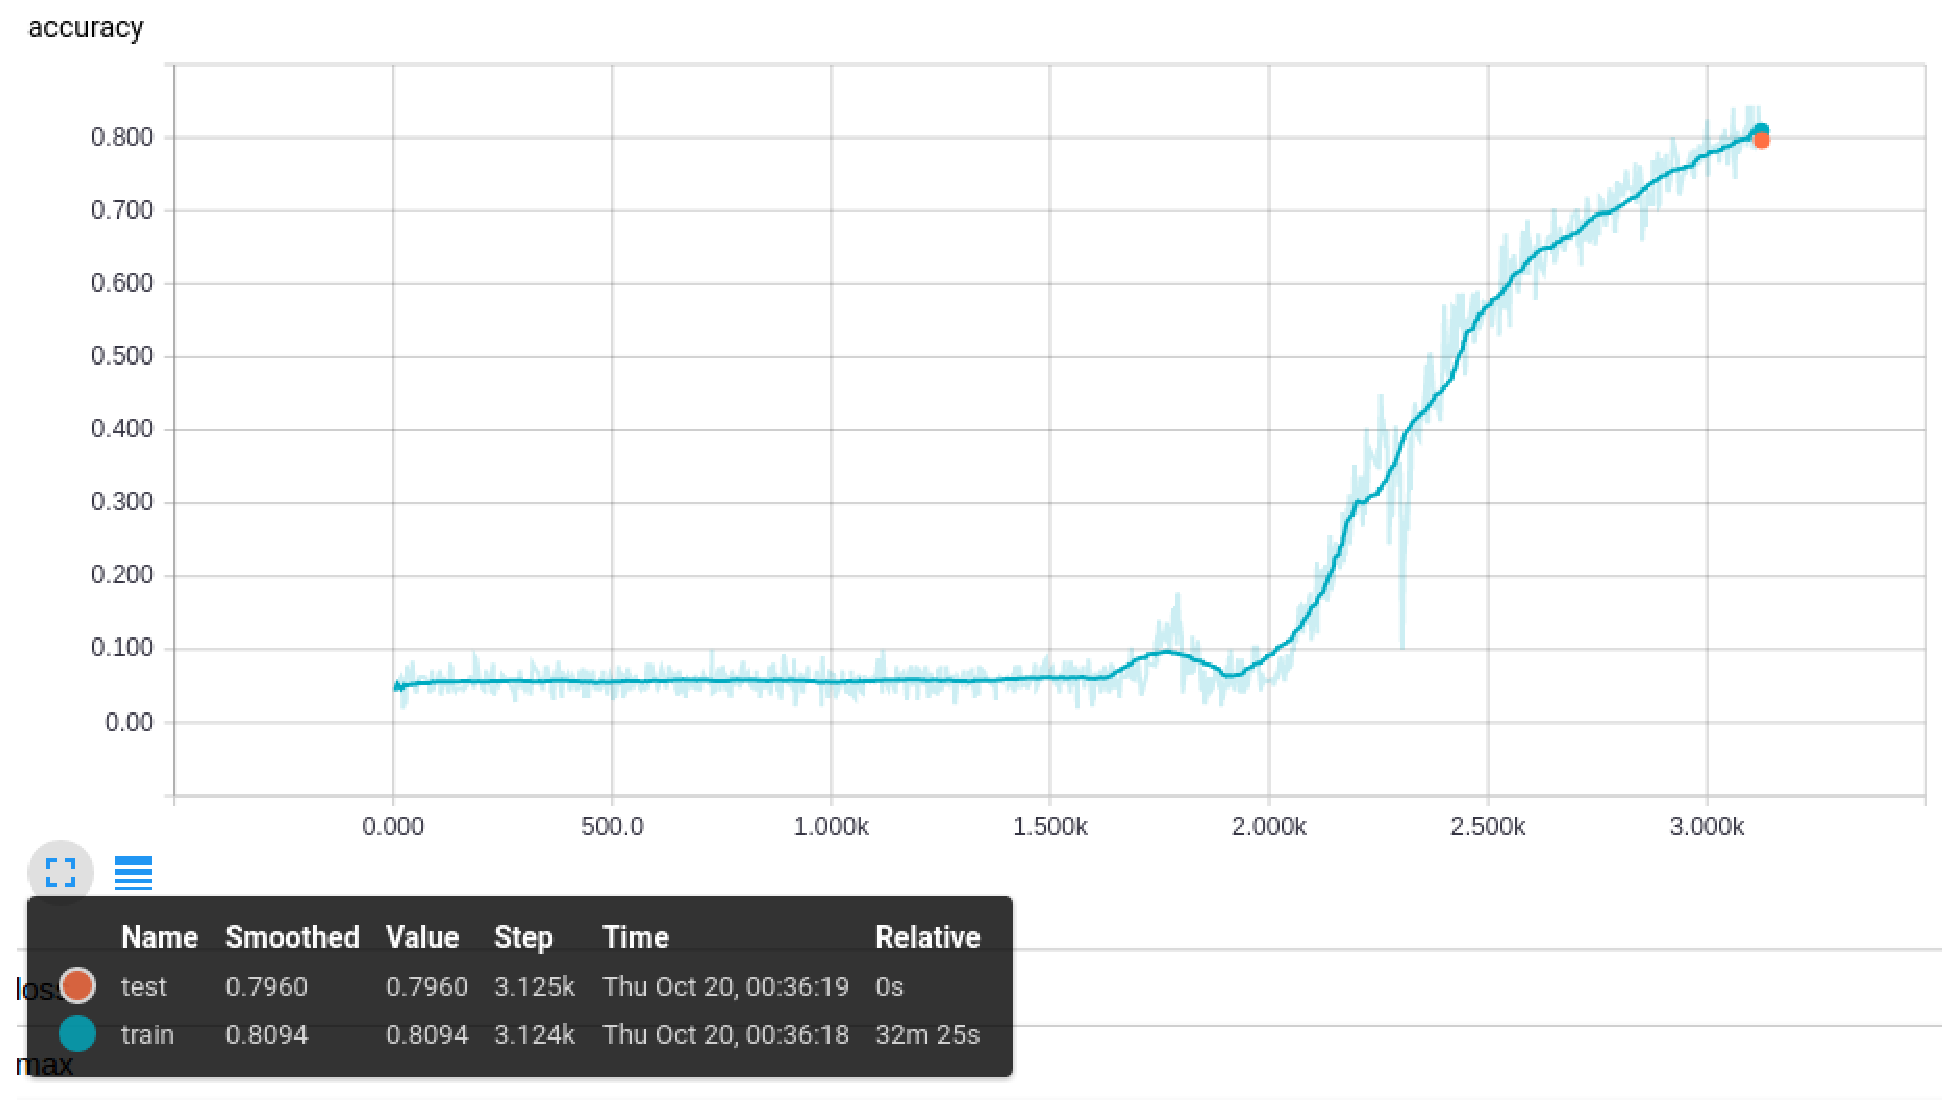
\includegraphics[scale=0.4]{imagens/accuracy_200k}
\caption{Gráfico da acurácia em relação ao número de passos para o
  treinamento da rede com 200 mil iterações.}
\label{fig:accuracy_200k}
\end{figure}

\begin{figure}[H]
\centering
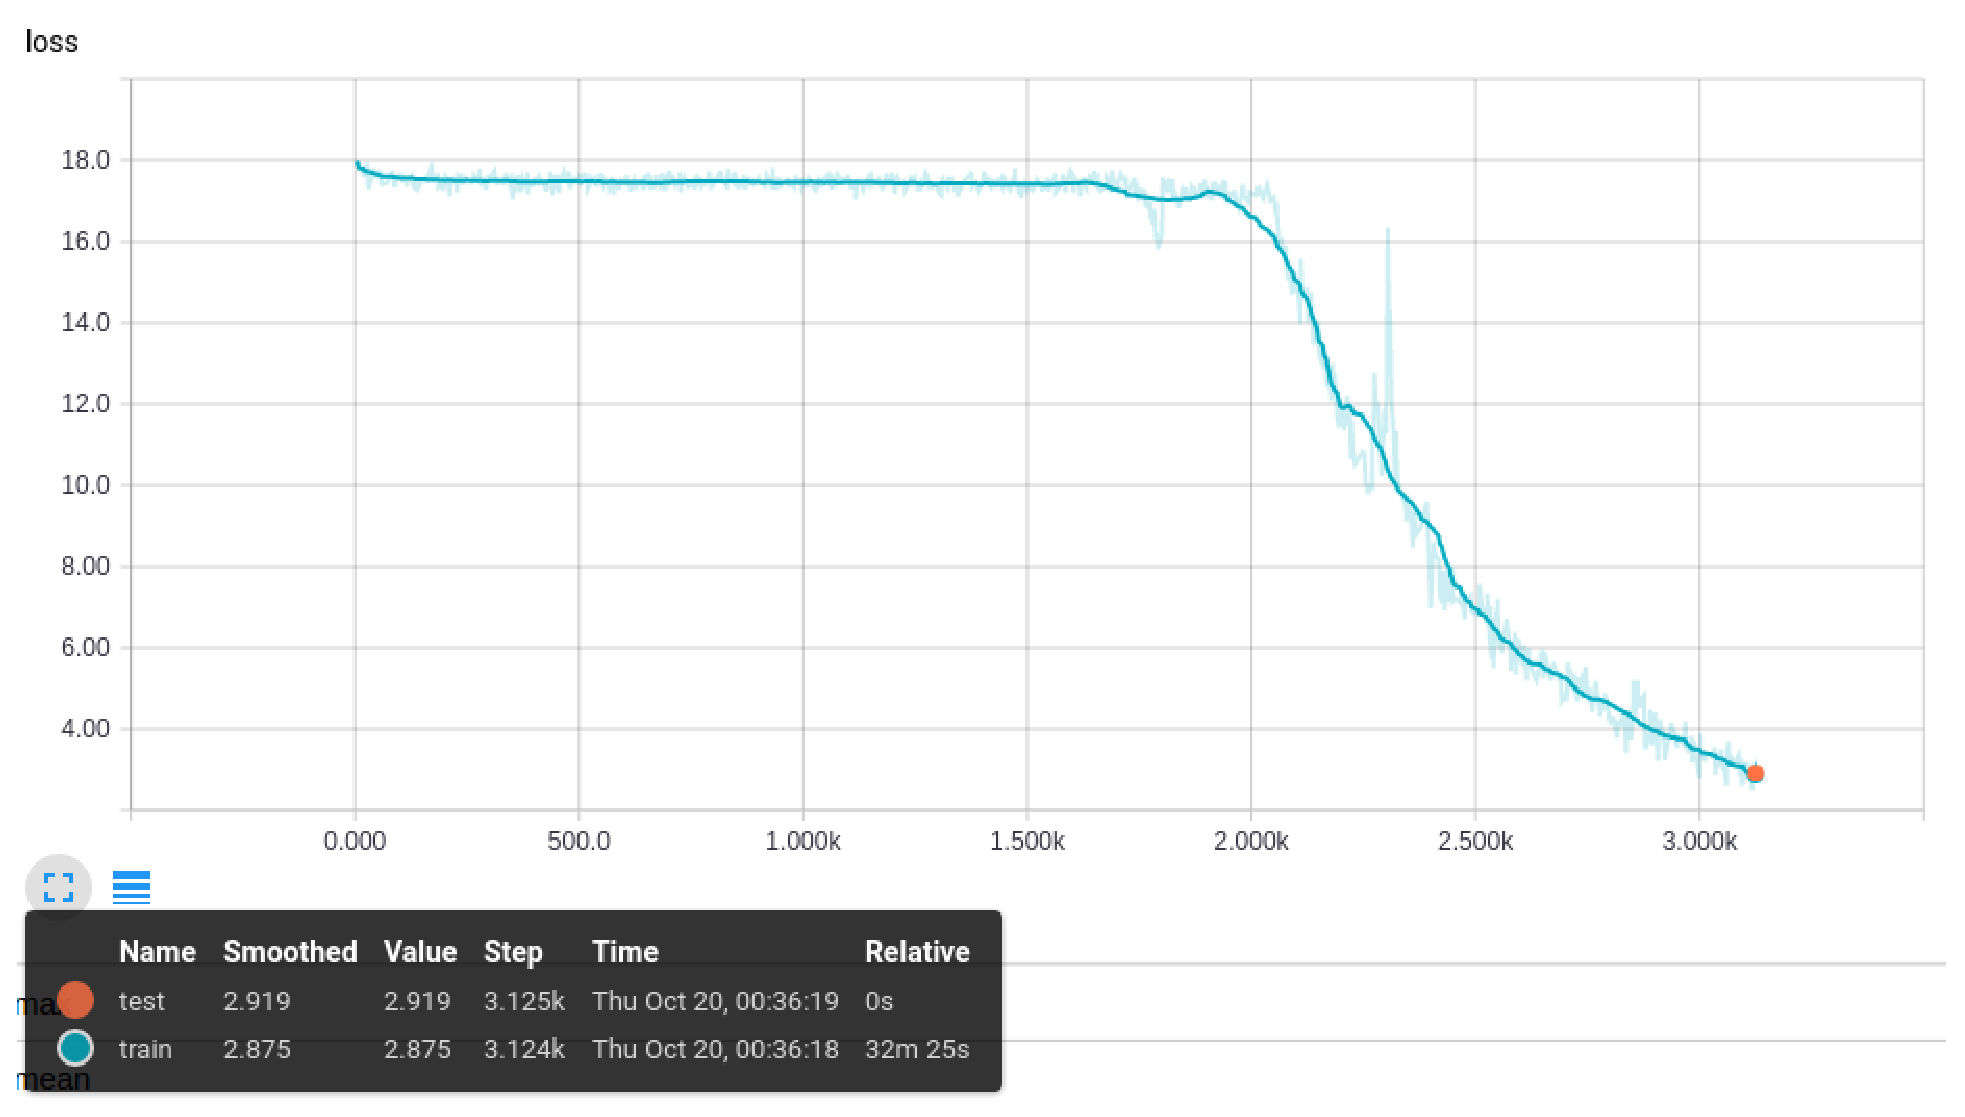
\includegraphics[scale=0.4]{imagens/loss_200k}
\caption{Gráfico da perda em relação ao número de passos para o
  treinamento da rede com 200 mil iterações.}
\label{fig:loss_200k}
\end{figure}

Mesmo com o bom resultado nos testes, foi notado uma falta de
estabilidade nos gráficos gerados. Analisando os gráficos de desvio
padrão dos valores de pesos e \textit{biases} das últimas camadas
convolucionais, percebe-se que alguns valores poderiam continuar
alterando se o treinamento continuasse por mais iterações.

\begin{figure}[H]
\centering
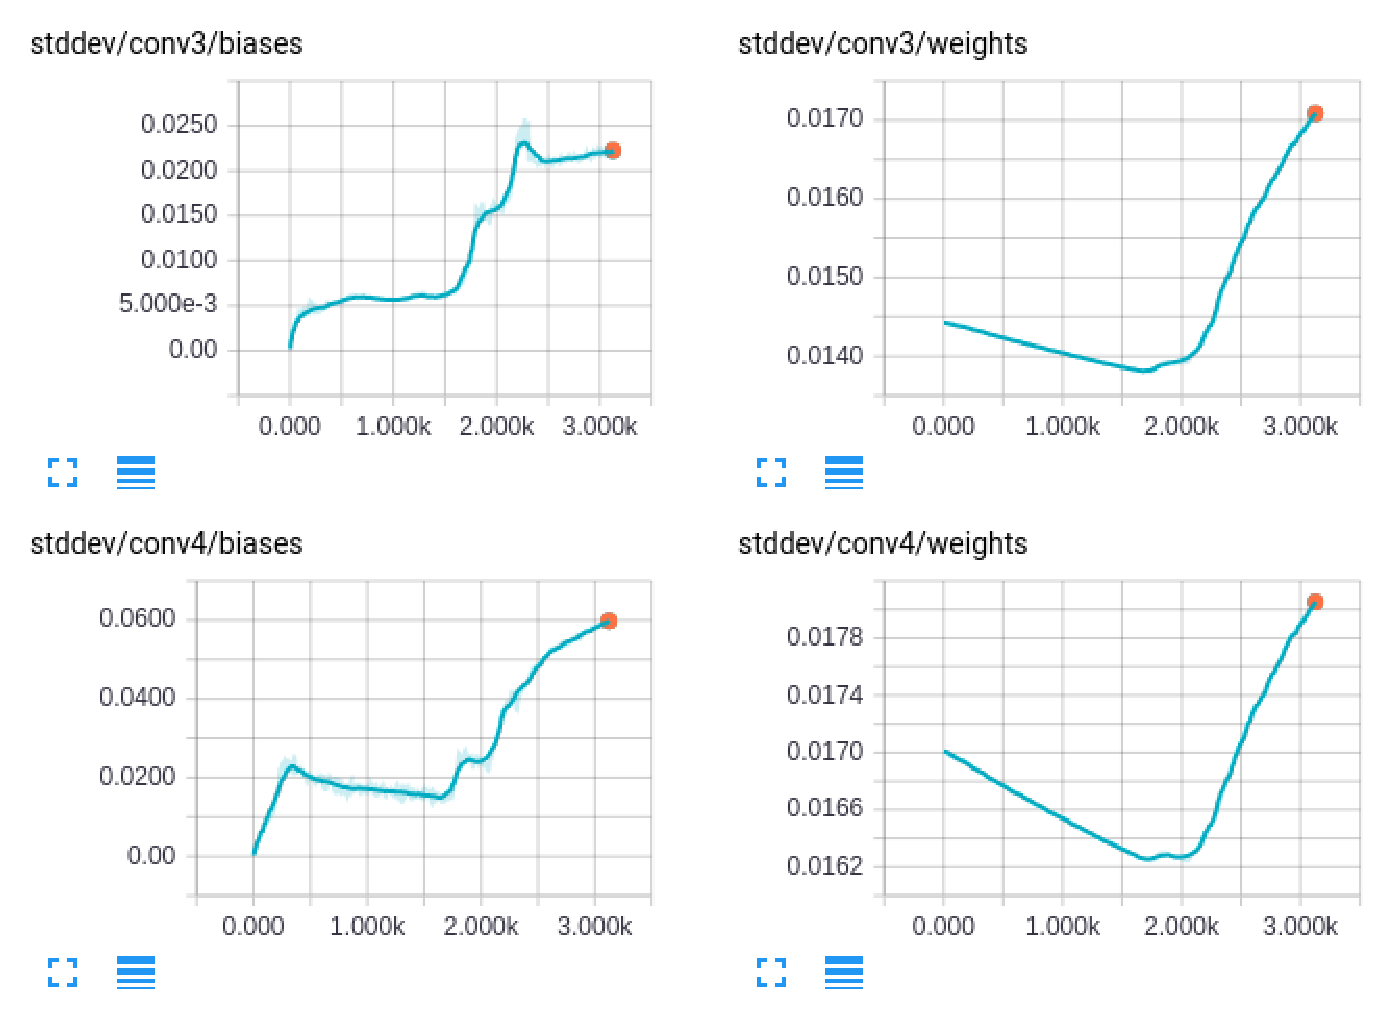
\includegraphics[scale=0.6]{imagens/stddev_200k}
\caption{Desvio padrão dos pesos e \textit{biases} em relação ao
  número de passos para o treinamento da rede com 200 mil iterações.}
\label{fig:stddev_200k}
\end{figure}

\section{Treinamento com 500 mil iterações}

Visto a instabilidade nos valores de gráficos no treinamento anterior,
a tentativa seguinte foi aumentar o número de iterações para 500 mil,
portanto 7.812 passos. O tempo total de treinamento foi de {\bf 1 hora
18 minutos e 23 segundos}.

Analisando os gráficos gerados com este treinamento, novamente o valor
da perda oscila entre 16,87 e 17,51 até um certo ponto. Dessa vez
é no passo número 2.922 (iteração 187.008) onde a perda começa a
decair. O mesmo acontece com a acurácia, ficando em torno de 6\% até o
passo 2.977 (iteração 190.528) quando começa a subir. Ao final do
treinamento foi alcançado o valor máximo de acurácia igual a {\bf
  98,75\%} no conjunto de treinamento, {\bf 81,37\%} no conjunto de
teste e um valor mínimo de perda igual a {\bf 0,36} para o conjunto de
treinamento, {\bf 13,52} para o conjunto de teste.

\begin{figure}[H]
\centering
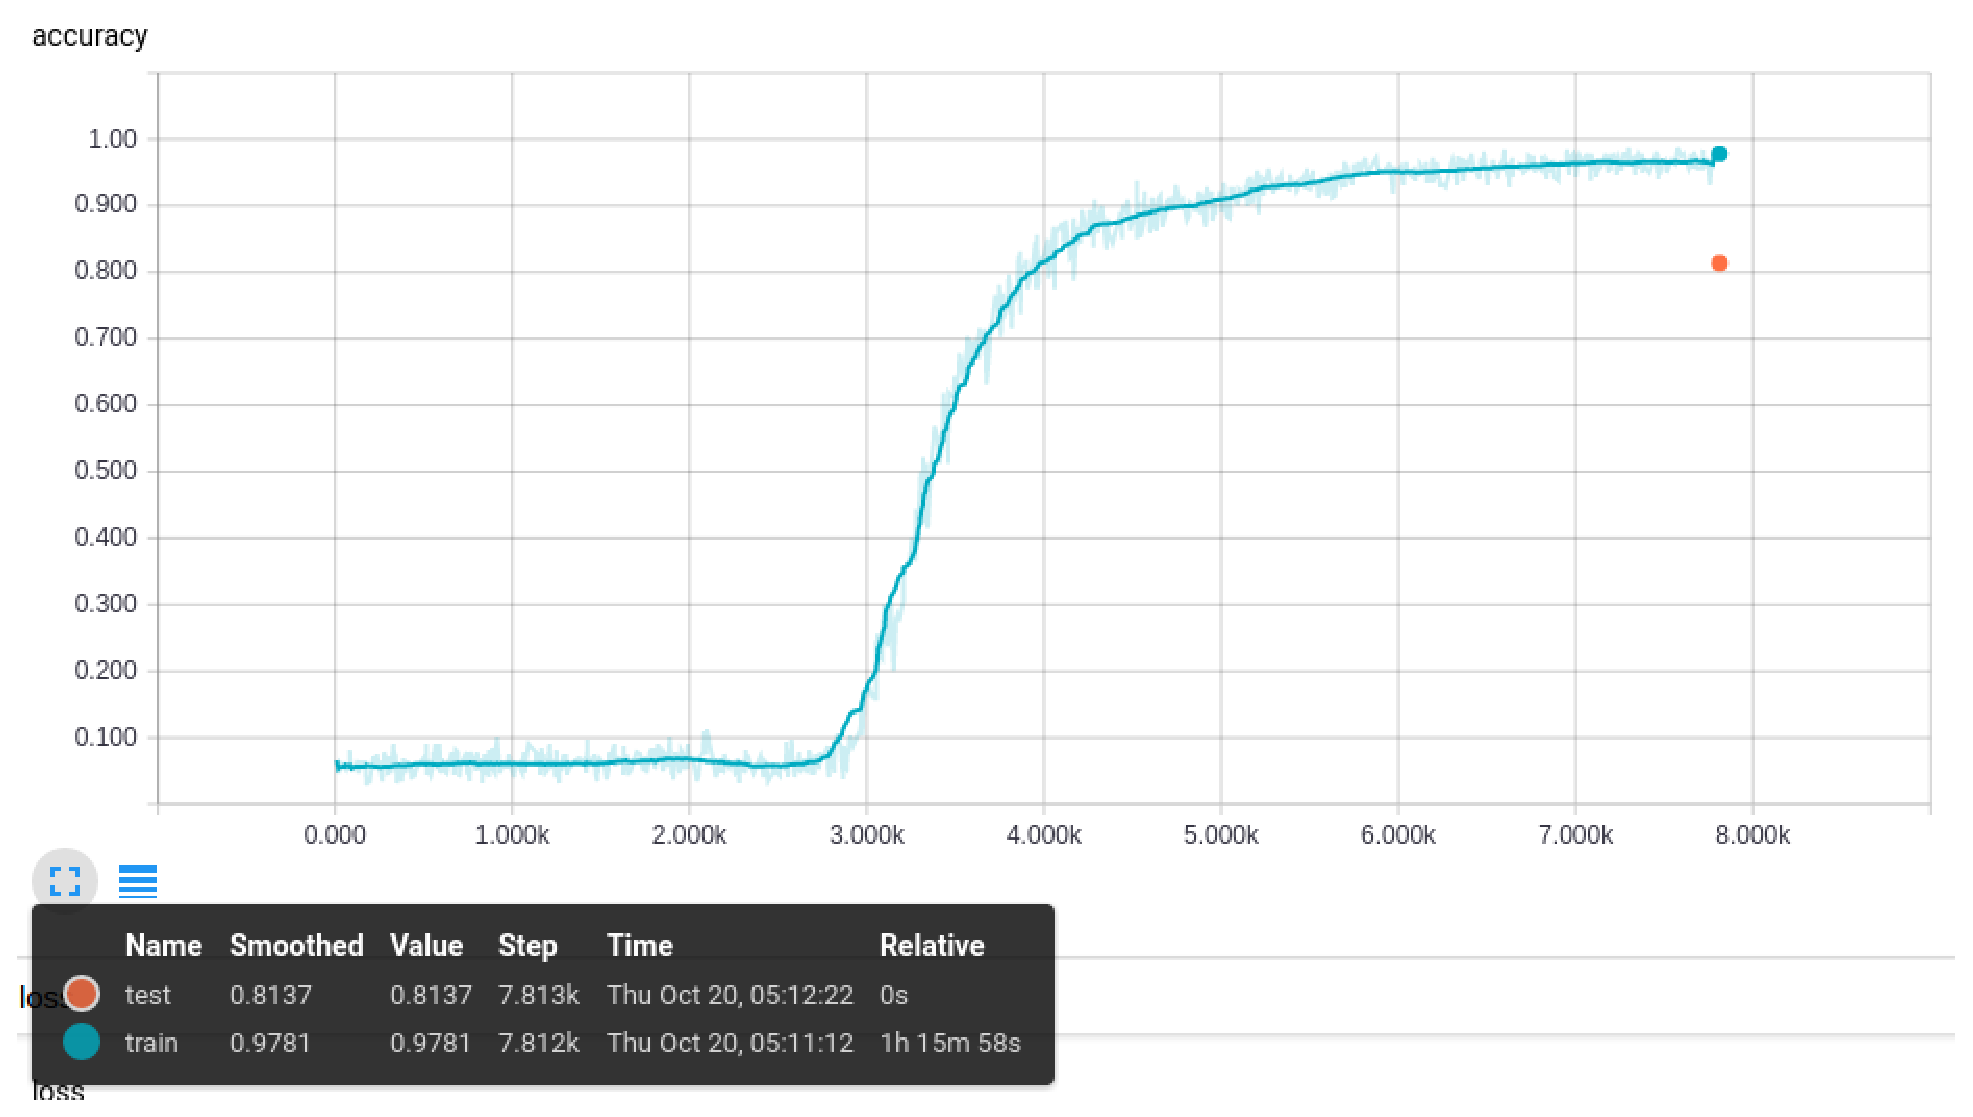
\includegraphics[scale=0.4]{imagens/accuracy_500k}
\caption{Gráfico da acurácia em relação ao número de passos para o
  treinamento da rede com 500 mil iterações.}
\label{fig:accuracy_500k}
\end{figure}

\begin{figure}[H]
\centering
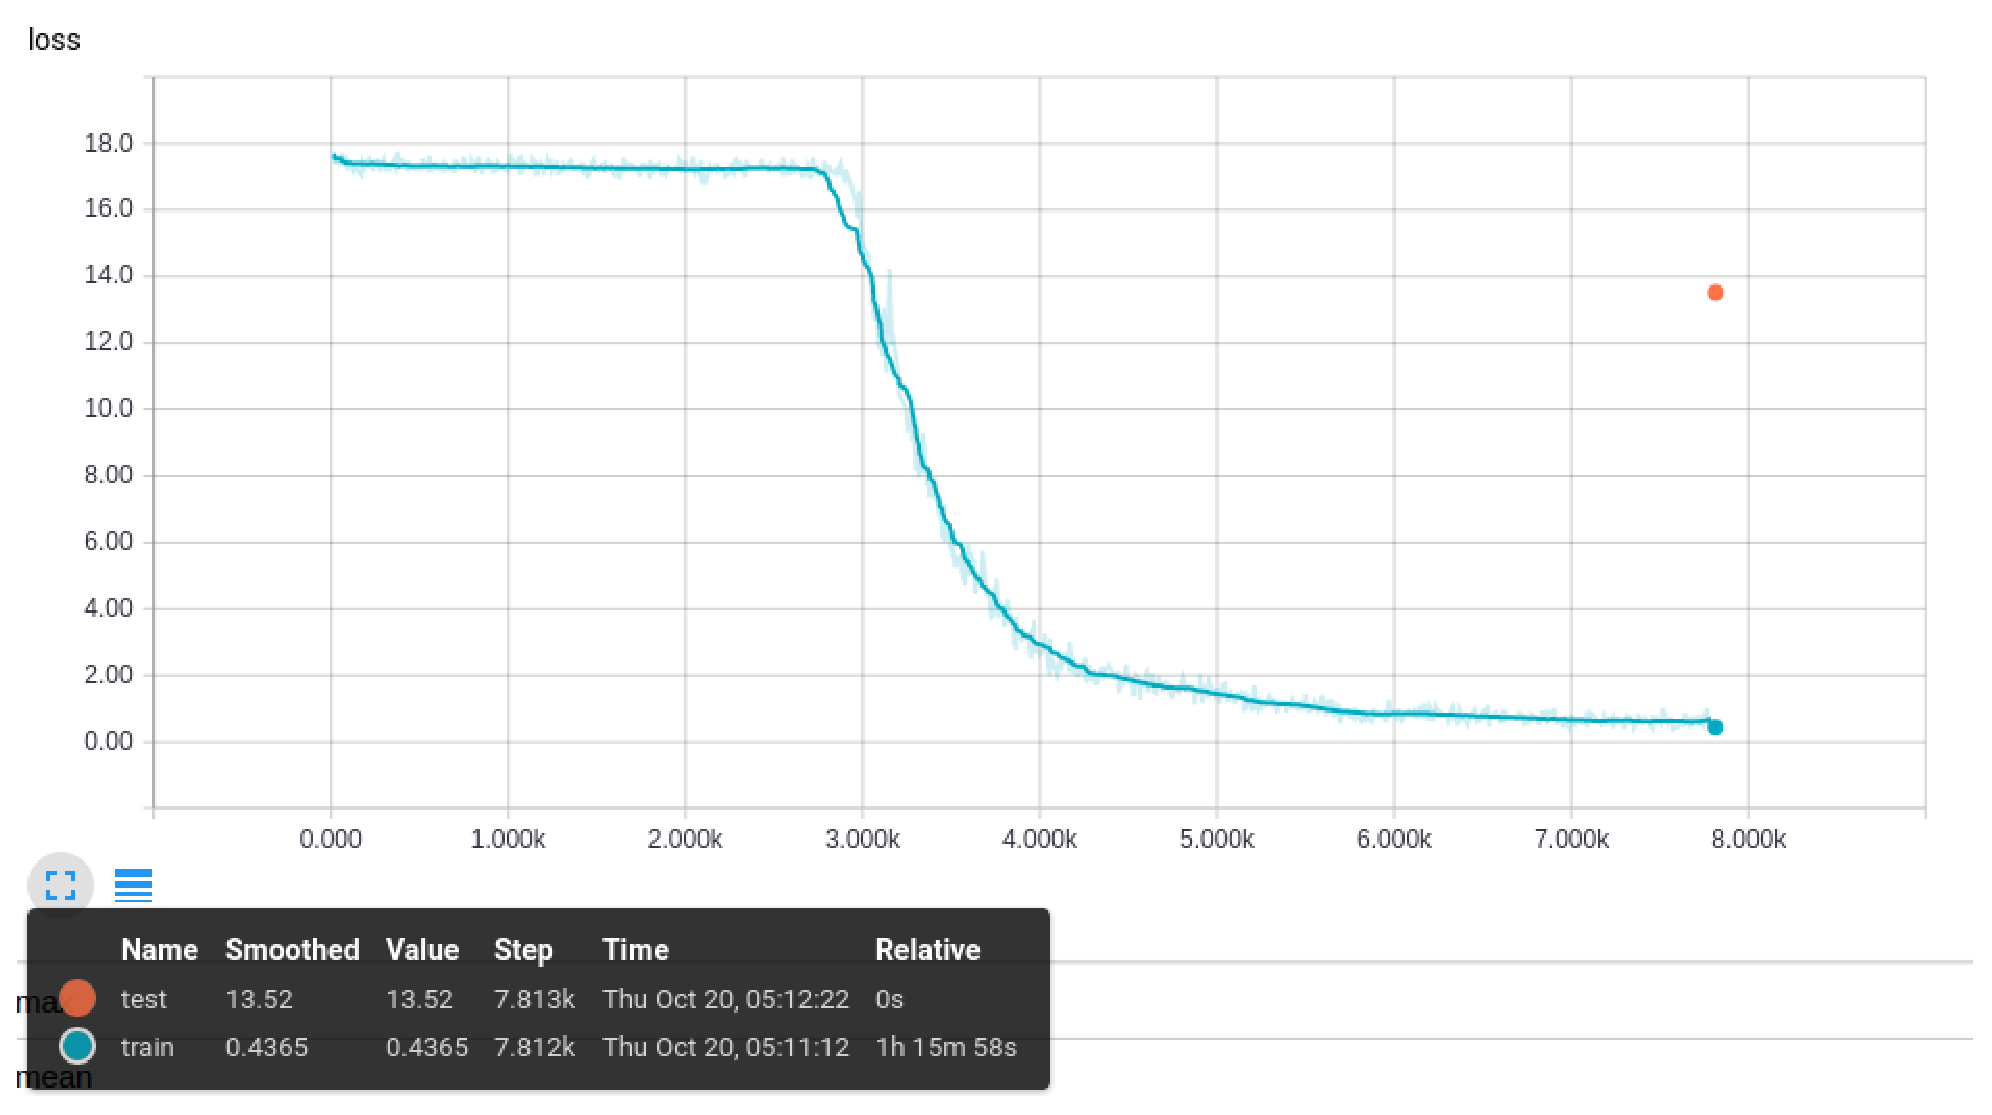
\includegraphics[scale=0.4]{imagens/loss_500k}
\caption{Gráfico da perda em relação ao número de passos para o
  treinamento da rede com 500 mil iterações.}
\label{fig:loss_500k}
\end{figure}

Analisando os resultados, é possível observar que o valor da perda
para o conjunto de treinamento é muito diferente do valor da perda
para o conjunto de teste. Também nota-se que a acurácia no conjunto de
treinamento chegou bem perto de 100\%. De acordo com a fundamentação
teórica, esses dois fatores podem ter sido causados pelo
\textit{overfitting} do modelo ao conjunto de dados do treinamento.

\section{Treinamento com 500 mil iterações e Dropout de 50\%}

Na tentativa de minimizar os problemas encontrados anteriormente, foi
realizado um terceiro treinamento. Foi visto que uma das técnicas de
regularização para minimizar o \textit{overfitting} é adicionando uma
camada de \textit{dropout} ao modelo. Nossa arquitetura já previa uma
camada de \textit{dropout}, no entanto o parâmetro de probabilidade de
mantimento das ativações estava configurado para 75\% (0,75). Para o
terceiro treinamento foi configurada a probabilidade do
\textit{dropout} para 50\% (0,5) e assim analisados os resultados. O
tempo total de treinamento foi de {\bf 1 hora 18 minutos e 53
  segundos}.


\begin{figure}[H]
\centering
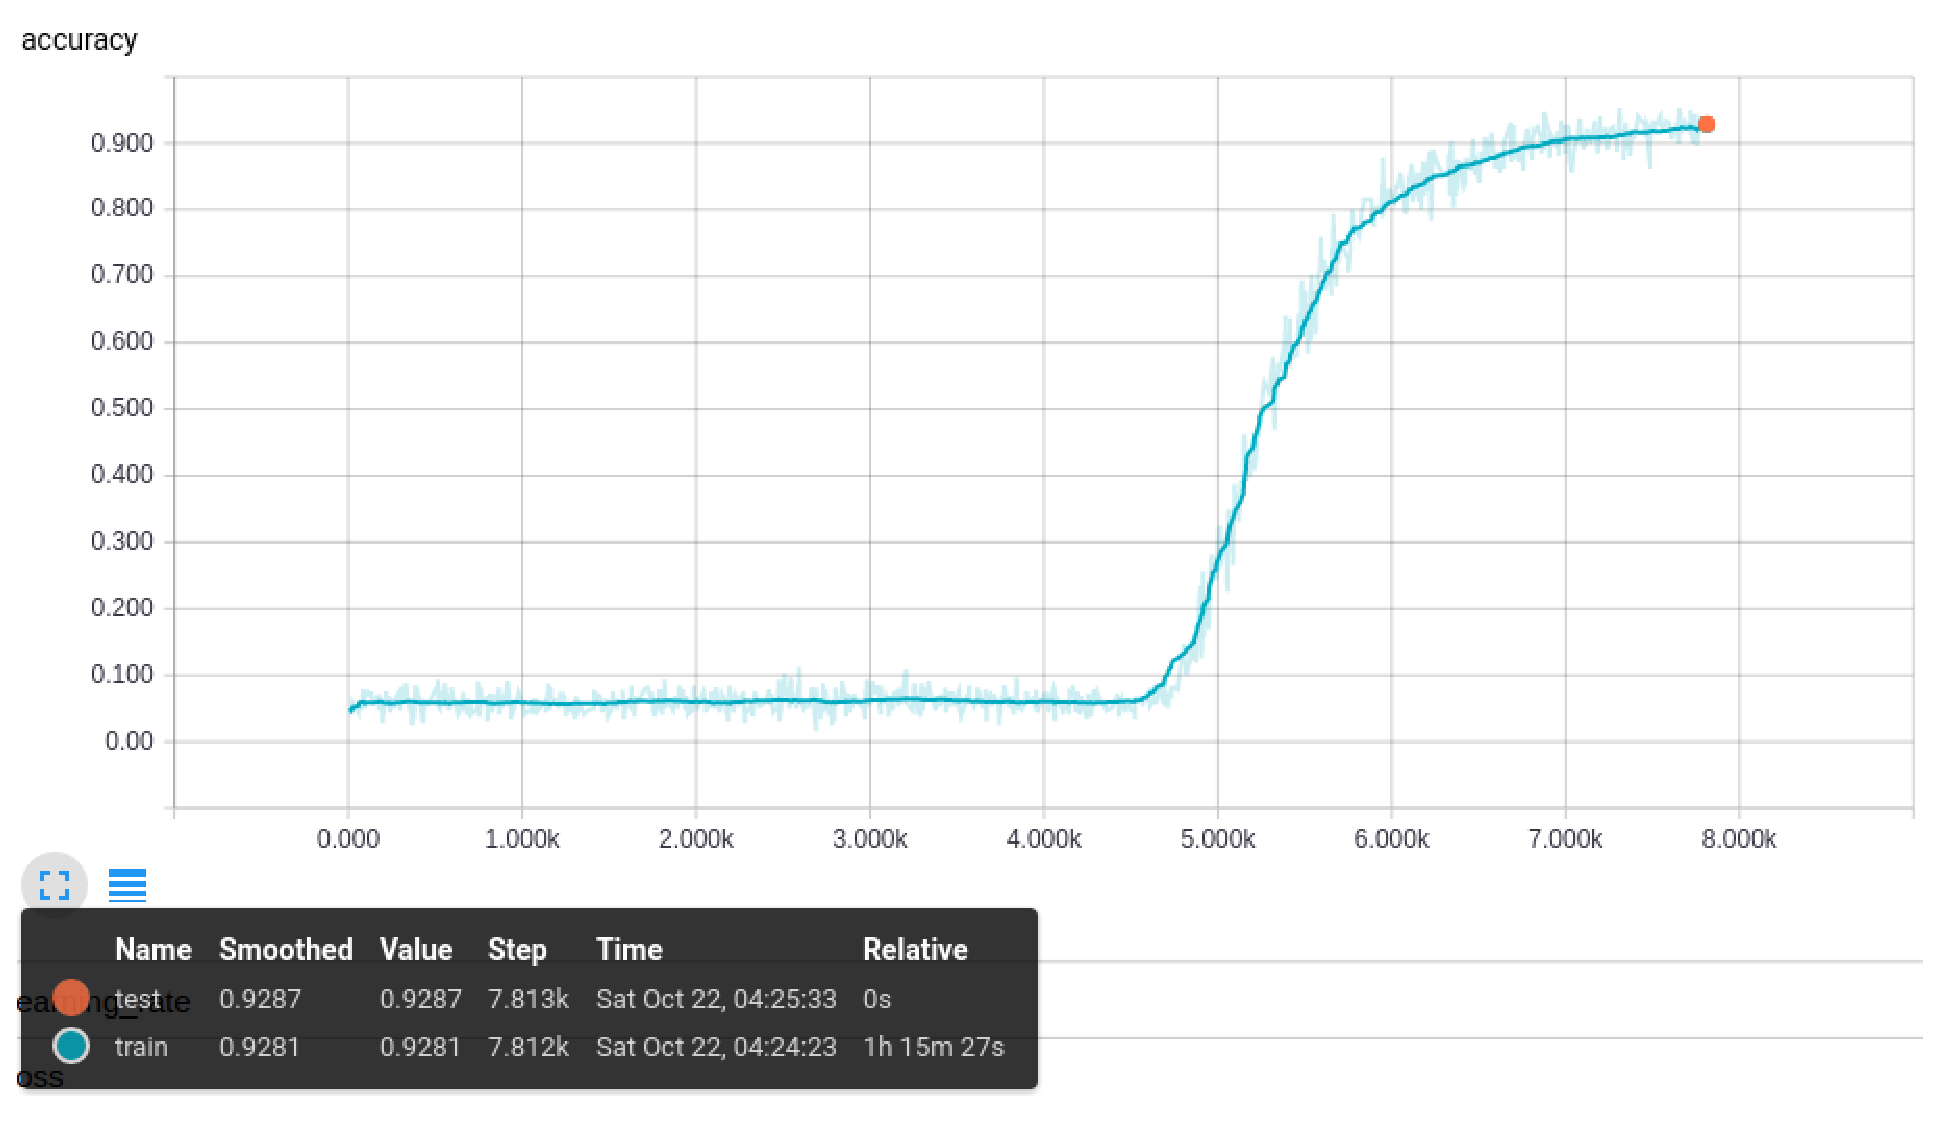
\includegraphics[scale=0.4]{imagens/accuracy_500k_dropout50}
\caption{Gráfico da acurácia em relação ao número de passos para o
  treinamento da rede com 500 mil iterações e probabilidade de
  \textit{dropout} igual a 50\%.}
\label{fig:accuracy_500k_dropout50}
\end{figure}

\begin{figure}[H]
\centering
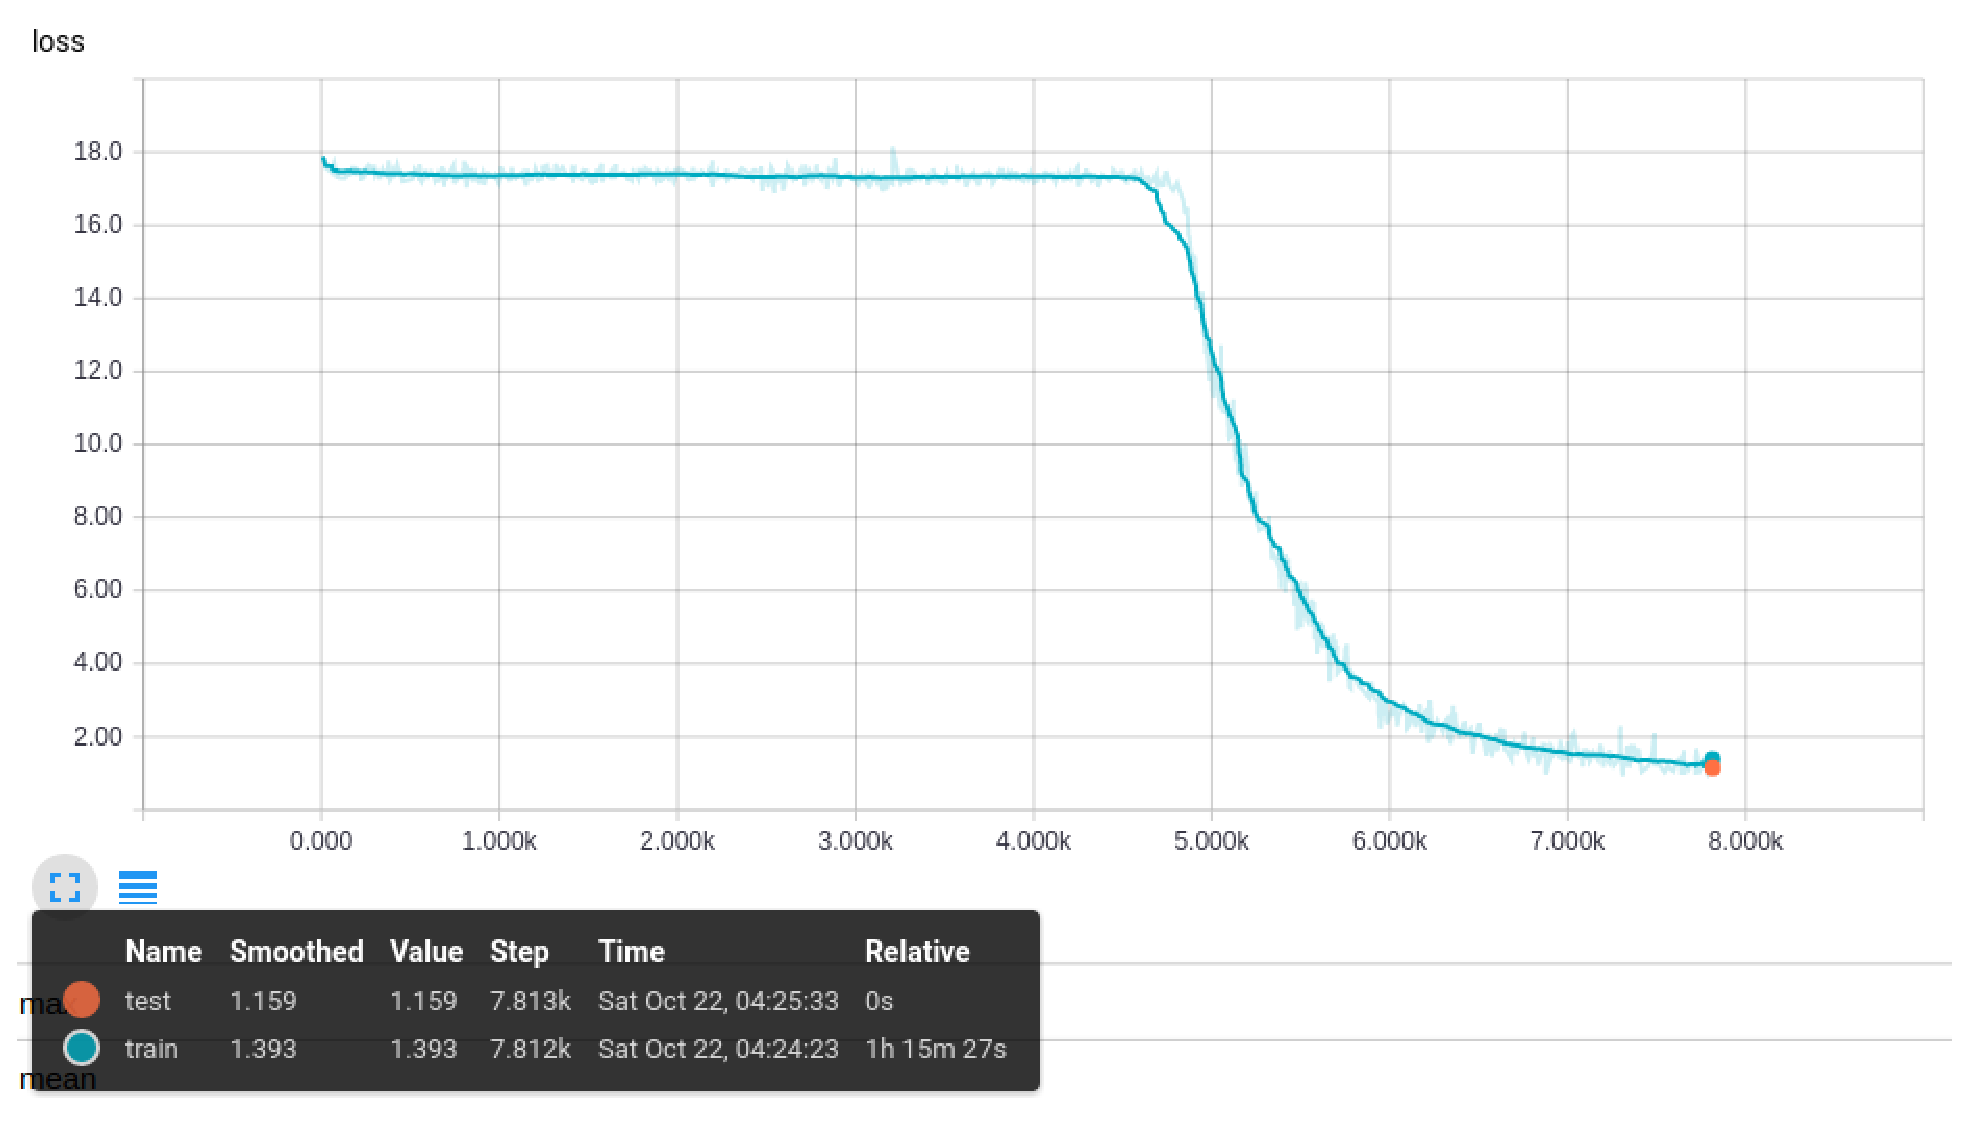
\includegraphics[scale=0.4]{imagens/loss_500k_dropout50}
\caption{Gráfico da perda em relação ao número de passos para o
  treinamento da rede com 500 mil iterações e probabilidade de
  \textit{dropout} igual a 50\%.}
\label{fig:loss_500k_dropout50}
\end{figure}

Ao final do treinamento foi alcançado o valor máximo de acurácia igual
a {\bf 95,31\%} no conjunto de treinamento, {\bf 92,87\%} no conjunto
de teste e um valor mínimo de perda igual a {\bf 0,93} para o conjunto
de treinamento, {\bf 1,15} para o conjunto de teste.

\section{Avaliação da acurácia em casos novos} \label{acuracia}

Como dito anteriormente na seção \ref{faseTeste}, o cálculo feito
para determinar a acurácia nos casos de teste não contemplam um acerto
completo de todas as letras em uma imagem de CAPTCHA. Por conta desse
fator e também para testar o modelo em imagens novas, foi desenvolvido
um script para carregar o modelo treinado. Esse script executa uma
sessão do modelo da mesma forma em que foi feito o treinamento na
seção \ref{treino}. A execução do teste foi mediante {\bf 18.000}
imagens novas para obter um resultado fiel a uma situação real de
reconhecimento de CAPTCHAs.

O cálculo final é simples, para cada imagem em que o modelo decifra
corretamente o texto, é incrementada uma variável {\bf acertos}. Ao
final da execução do teste para cada imagem, é dividido o número de
acertos pelo total de imagens fornecidas. A taxa de acurácia alcançada
ao executar a avaliação foi de {\bf 79,65\%}, ou seja {\bf 14.337}
imagens reconhecidas completa e corretamente.

\section{Resultados}

De acordo com os testes realizados, a configuração de alguns
parâmetros no treinamento foram essenciais para eficácia do sistema
proposto.

\begin{table}[H]
\begin{center}
\begin{tabular}{|p{2.3cm}|p{2.3cm}|p{2.3cm}|p{2.3cm}|}
\hline
\textbf{} & \textbf{200k it.} & \textbf{500k it.} & \textbf{500k it. e 50\% \textit{dropout}} \\
\hline
Acurácia (teste) & {\bf 79,6\%} & {\bf 81,37\%} & {\bf 92,87\%} \\
\hline
Acurácia (treinamento) & 84,38\% & 98,75\% & 95,31\% \\
\hline
Perda (teste) & 2,91 & 13,52 & 1,15 \\
\hline
Perda (treinamento) & 2,50 & 0,36 & 0,93 \\
\hline
\end{tabular}
\caption{Desempenho geral do sistema.}
\label{tab:system_efficency}
\end{center}
\end{table}

\begin{table}[H]
\begin{center}
\begin{tabular}{|p{5cm}|p{5cm}|}
\hline
\textbf{} & \textbf{Avaliação do modelo de 500k it. e 50\% \textit{dropout}} \\
\hline
Acurácia & {\bf 79,65\%} \\
\hline
Imagens corretamente classificadas & 14.337 \\
\hline
Total de imagens & 18.000 \\
\hline
\end{tabular}
\caption{Avaliação em casos novos do modelo treinado com 500 mil
  iterações e 50\% de \textit{dropout}.}
\label{tab:system_evaluation}
\end{center}
\end{table}

Com a execução do script de acurácia citado na seção \ref{acuracia},
foram identificados diversos casos complexos em que o modelo teve
êxito no reconhecimento do texto completo.

\begin{figure}[H]
\centering
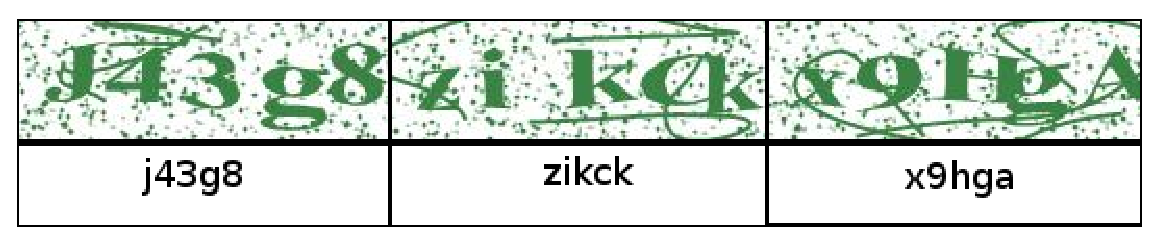
\includegraphics[scale=0.8]{imagens/complex_cases}
\caption{Exemplos de casos complexos.}
\label{fig:complex_cases}
\end{figure}

Para os casos complexos demonstrados na figura
\ref{fig:complex_cases}, o reconhecedor acertou o texto completo da
imagem. Na primeira imagem é possível observar a semelhança entre uma
letra ``g'' e o dígito ``8''. Diante da proximidade entre as letras da
segunda imagem, o modelo poderia ter classificado a penúltima letra
como um ``q'' ao invés do ``c'' que foi a letra correta. Novamente
é perceptível a proximidade entre as letras na terceira imagem. Abaixo
das imagens se encontram os textos reconhecidos pelo modelo em cada
caso respectivamente.

Contudo também foram observados casos em que o modelo não teve sucesso
no reconhecimento do texto completo. Devido a semelhança de alguns
caractéres, o modelo reconheceu parcialmente o texto de algumas
imagens apresentadas.

\begin{figure}[H]
\centering
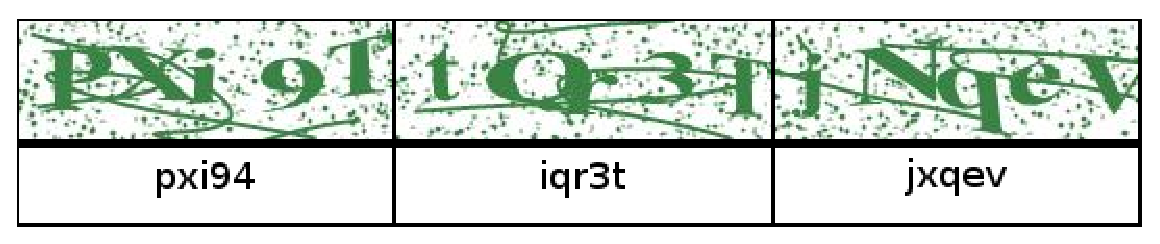
\includegraphics[scale=0.8]{imagens/harder_cases}
\caption{Exemplos de casos complexos em que o reconhecedor acertou
  parcialmente o texto da imagem.}
\label{fig:harder_cases}
\end{figure}

Na primeira imagem da figura \ref{fig:harder_cases} é possível observar
que o modelo confundiu a letra ``T'' maiúscula com um dígito ``4''. Na
segunda imagem, mesmo com a sobreposição dos caractéres ``Q'' e ``r''
no meio da imagem, esses caractéres foram reconhecidos
corretamente. Enquanto o primeiro carctere ``t'' no início da imagem
foi erroneamente reconhecido como uma letra ``i''. Na terceira imagem
a letra ``N'' maiúscula foi reconhecida erroneamente como uma letra
``x''. Abaixo das imagens se encontram os textos reconhecidos pelo
modelo em cada caso respectivamente.

\chapter{Conclusões}

\bibliography{ref}

\end{document}
